\section{Experiment}
We demonstrate EMO's empirical performance as a continual fine-tuning method upon pre-trained LMs. In Sec.~\ref{sec:generation}, we compare EMO against MLE as well as other training criteria on a diverse range of language modeling datasets. In Sec.~\ref{sec:nlu_all}, we 
investigate the effectiveness of EMO on natural language understanding tasks under the few-shot in-context learning setting based on LLMs with various scales. The evaluation of EMO in instruction-tuning scenario is deferred to Appendix~\ref{appendix:instruction}.
\subsection{Language Modeling}
\label{sec:generation}
% In this subsection, our primary goal is to evaluate the distribution matching ability, i.e., the degree of distributional similarity between texts generated by the model and those produced by humans, by fine-tuning pre-trained language models on unlabelled textual corpora from various domains.
\subsubsection{Setup}
\label{sec:main_setup}
\paragraph{Task Definition and Evaluation Metric} 
To gauge the quality of the learned model distribution after fine-tuning on a domain-specific corpus, we provide the model with a prefix and request it to continue with a segment of text that should ideally be similar to the reference text. We adopt Mauve~\citep{mauve} as the main evaluation metric, which compares the generated continuation against human text by calculating the area under
the KL divergence curve and has seen wide usage in open-ended text generation~\citep{tailr,mixce,meister-etal-2023-efficacy}.
%In the experiments, the lengths of the prefix and the generated continuation are set as 32 and 128
\paragraph{Pre-trained Language Models}
We utilize two representative decoder-only Transformer~\citep{transformer} language models, namely GPT-2~\citep{gpt2} and OPT-125M~\citep{opt}, as $Q_{\theta}$, and fine-tune them using distinct training criteria including EMO and several recently proposed methods discussed below.
\paragraph{Baselines}
Aside from MLE, we also compare with the following baselines, which aim to address the shortcomings of MLE by introducing novel divergence measures~(or approximated variants) as their training objectives: 
(1)~TaiLr~\citep{tailr} adopts the total variation distance~\citep{van2014probability} as a more robust measure between probability distributions and uses its token-level factorization as the training objective. (2)~MixCE~\citep{mixce} penalizes low-quality samples by leveraging an approximated version of reverse cross-entropy. For TaiLr and MixCE, we follow the implementations from their corresponding official codebase.
More discussions regarding these baselines can be found in the Appendix~\ref{appendix:baseline_detail}.
\paragraph{Datasets}
We use 6 English textual corpora from 5 different domains for comprehensive evaluation:(1)~WikiText-2 and WikiText-103~\citep{wikitext} are two commonly used language modeling benchmarks consisting of high-quality Wikipedia articles. (2)~WebText$_{\text{test}}$~\citep{webtext} is the test set of the official WebText dataset from OpenAI, that was used to train GPT-2. 
(3)~Penn Tree Bank~(PTB)~\citep{ptb} contains Wall Street Journal material in financial domain. (4)~ WritingPrompts~\citep{wp} features text from the writing prompts forum of Reddit. (5)~AG News~\citep{agnews} is a collection of news articles from diverse domains, e.g., business, sports, and science. The statistics of each dataset are deferred to the Appendix~\ref{appendix:a1}.

\paragraph{Training Details}
We fine-tune GPT-2 and OPT-125M for 3 epochs on the training set of each dataset and save the model checkpoint with the lowest validation loss. We use the AdamW~\citep{adamw} optimizer with a learning rate of 5e-5. The batch size is fixed as 32 for all experiments. The maximum input length during training is set to 256. For TaiLr and MixCE that involve weighting coefficient, we conduct a hyperparameter sweep within $\{0.9, 0.8, 0.7\}$. EMO does not necessitate any hyperparameter tuning. 

\paragraph{Decoding Algorithm}
To gauge the quality of the learned model distribution $Q_{\theta}$ in a faithful way~\citep{eikema2020map}, we employ unbiased sampling~(also known as ancestral sampling) as the primary decoding algorithm throughout the experiments. The length of prefixing and generated tokens for each dataset can be found in Appendix \ref{appendix:a1}. We repeat the sampling process 5 times for each prefix and report the average 
Mauve score.
\subsubsection{Main Results}
\begin{table}[h!]
    \centering
    \footnotesize
    \caption{Unbiased sampling results~(Mauve$\uparrow$) of models fine-tuned by EMO as well as compared baselines. Numbers are the mean of 5-run sampling, aggregated over 3 different random seeds. \textbf{Bold} numbers indicate the results are significantly better than MLE with $p$-value $<$ 0.001.}
    \begin{tabular}{cc|cccccc}
    \toprule
    \textbf{Model}                     & \textbf{Objective} & \textbf{WikiText2}    & \textbf{WikiText103}  & \textbf{WebText$_{\text{test}}$}  & \textbf{PTB}           & \textbf{WritingPrompts} & \textbf{AG}       \\
    \midrule
    \multirow{4}{*}{GPT-2}    & MLE       & 77.5          & 77.1          & 75.5          & 76.1          & 83.6           & 75.0          \\
                              & TaiLr     & 79.6          & 78.0          & 76.5          & 73.8          & 84.1           & 75.8          \\
                              & MixCE     & 78.3          & 77.6          & 76.3          & 76.9          & 82.7           & 76.6          \\
                              & EMO    & \textbf{87.5} & \textbf{82.1} & \textbf{80.5} & \textbf{79.6} & \textbf{87.4}  & \textbf{84.9} \\
    \midrule
    \multirow{4}{*}{OPT$_{\text{125M}}$} & MLE       & 77.2          & 75.8          & 74.7          & 83.6          & 84.1           & 82.1          \\
                              & TaiLr     & 78.4          & 75.2          & 74.2          & 82.2          & 83.4           & 81.8          \\
                              & MixCE     & 78.6          & 75.4          & 75.3          & 81.5          & 83.5           & 83.2          \\
                              & EMO    & \textbf{82.9} & \textbf{81.0} & \textbf{80.7} & \textbf{86.1} & \textbf{87.9}  & \textbf{84.8} \\
    \bottomrule
    \end{tabular}
    \label{table:mauve}
\end{table}
Table~\ref{table:mauve} summarizes the unbiased sampling results of GPT-2 and OPT-125M fine-tuned with different training objectives on six datasets. We can clearly observe that EMO consistently 
outperforms MLE and other recently proposed training criteria across various domains. Although TaiLr and MixCE both leverage new distance measures that have theoretical advantages over forward cross-entropy, they suffer from either a mild assumption about the model's training dynamics or degeneration into a regularized version of forward cross-entropy. Therefore, they still exhibit the same drawbacks of MLE stated in Sec.~\ref{sec:deficiency}. 
In contrast, EMO effectively manifests its theoretical advantages and leads to language models with more human-like distribution. For more quantitative results about the learned model distribution please refer to Appendix \ref{appendix:p_r}.
\subsubsection{Experiment with Oracle Data Generator}
In addition to the setting where we only have access to training data sampled from unknown distribution, in this subsection we seek to analyze more fine-grained distributional properties of models trained with different criteria. Specifically, we 
use training data sampled from an orcale GPT-2-Large model whose distribution $P$ is known. We use the GPT-2-output dataset consisting of 250,000/5,000/5,000 paragraphs in the training/validation/test set generated via unbiased sampling.
\paragraph{Setup}
Apart from Mauve for measuring the sequence-level similarity between texts sampled from the learned and oracle model, we also incorporate model's test set perplexity PPL$_{\text{test}}$ , the oracle model's perplexity PPL$_{\text{oracle}}$~(calculated using oracle model on model-generated texts) and ROUGE-1/L~\citep{rouge} that evaluate the learned distributions from different perspectives. PPL$_{\text{test}}$ is commonly adopted as a quantitative measure of model's \textit{recall}. PPL$_{\text{oracle}}$ emphasizes more on \textit{precision} by penalizing generations $\bm{x}$ from $Q_{\theta}$ that are unlikely to be produced by the oracle model $P$, i.e., $P(\bm{x})$ is low, While ROUGE score focuses on \textit{recall} by rewarding high n-gram overlap. For each training method, we fine-tune GPT-2 using the same experimental setting 
as described in Sec.~\ref{sec:main_setup}.
\begin{table}[h!]
    \centering
    \small
    \caption{Unbiased sampling results of GPT-2 fine-tuned with different training criteria. Numbers are the mean of 5-run sampling, aggregated over 3 different random seeds. \textbf{Bold} numbers indicate the results are significantly better with $p$-value $<$ 0.001.}
    \begin{tabular}{cccccc}
    \toprule
    \textbf{Methods} & \textbf{PPL$_{\text{test}}\downarrow$} & \textbf{PPL$_{\text{oracle}}\downarrow$} & \textbf{Mauve$\uparrow$}        & \textbf{ROUGE-1$\uparrow$}       & \textbf{ROUGE-L$\uparrow$}       \\
    \midrule
    MLE   &\textbf{70.1}  & 114.46      & 77.5 & 34.59 & 29.85 \\
    TaiLr &73.5  & 95.22       & 77.4 & 34.95 & 30.09 \\
    MixCE &74.4  & 79.46       & 78.4 & 35.31 & 30.26 \\
    EMO &74.9  & \textbf{55.85}                & \textbf{83.4}          &\textbf{37.37}          & \textbf{31.17}          \\
    \bottomrule
    \end{tabular}
    \label{table:oracle}
\end{table}
\paragraph{Results}
We report the performance of EMO as well as baseline methods in Table \ref{table:oracle}. The results consistently reveal that EMO outperforms all baseline methods across all evaluation metrics, except for PPL$_\text{test}$. Notably, EMO exhibits a significantly reduced PPL$_{\text{oracle}}$ compared to the baseline methods, demonstrating its effective mitigation of the overestimation issue associated with low-quality text in prior divergence measures. The awareness of diversity within the range of plausible tokens in addition to the gold token is naturally reflected in EMO's higher PPL$_\text{test}$. As indicated by the highest MAUVE score, EMO strikes the best balance between recall and precision, suggesting that utilizing a well-structured probability distribution distance metric as the optimization objective enables the language model to effectively balance precision and recall.
\subsection{language understanding}
\label{sec:nlu_all}
% In this subsection, we explore the impact of a lightweight continual fine-tuning stage upon language models using different training objectives on their downstream performance.
\subsubsection{Setup}
\paragraph{Pre-trained LLMs} We adopt LLaMa-7B and LLaMa-13B~\citep{llama1} as the pre-trained LLMs. More results using LLaMa2-7B/13B~\citep{llama2} are deferred to Appendix~\ref{appendix:a3} due to space limits.
\paragraph{Continual Fine-tuning} We perform continual fine-tuning on WikiText-103 using EMO and all baseline methods compared in Sec.~\ref{sec:generation}. The corpus used for fine-tuning is substantially smaller~(0.1B v.s. 1.4T tokens) than the corpus used for pre-training LLMs, therefore being much more efficient and resource-friendly. Using the same corpus for lightweight fine-tuning, our goal here is to explore the effect of different training objectives on downstream performance. For EMO, $\bm{E}$ is initialized from the pre-trained language modeling head and stay fixed during fine-tuning.
\paragraph{Downstream Tasks} We evaluate the fine-tuned models across an array of NLU tasks using in-context learning. Specifically, we use the following datasets: Tweet Emotion~\citep{tweetemotion}, TREC~\citep{trec1,trec2}, SST-2~\citep{sst2}, Subj~\citep{subj}, Customer Review~\citep{cr}, Rotten Tomatoes~\citep{rt}, AG News~\citep{agnews}, and MMLU~\citep{mmlu}. Following \cite{sail,wu-etal-2023-openicl}, A pre-trained dense retriever is used to find the 8 most similar samples as the in-context demonstrations for all datasets except for MMLU, where a fixed 5-shot demonstrations are used following common practice. Prompt templates and statistics for each task can be found in 
 Appendix~\ref{appendix:a2}.
\subsubsection{Main Results}
\begin{table}[h!]
    \centering
    \footnotesize
        \caption{Downstream performance of LLaMa-7B/13B  fine-tuned with different training objectives.}
    \begin{tabular}{cc|cccccccc}
        \toprule
        \textbf{Models}             & \textbf{Methods} & \textbf{TE} & \textbf{SST-2} & \textbf{TREC} & \textbf{Subj} & \textbf{CR} & \textbf{RT} & \textbf{AG} & \textbf{MMLU} \\
        \midrule
        \multirow{5}{*}{LLaMa-7B} & Pre-trained      & 54.1                    & 94.7           & 77.8          & 74.7          & 91.4        & 90.0                     & 85.6              & 31.4 \\
                                    & MLE              & 53.5                    & 94.8           & 79.0          & 74.5          & 92.0        & 91.8                     & 85.5              & 31.9 \\
                                    & TaiLr            & 56.2                    & 94.9           & 79.6          & 76.8          & 92.0        & 91.9                     &86.3              & 33.2 \\
                                    & MixCE            & 60.0                    & 95.0           & 81.2          & 78.5          & 92.0        & 91.8                     & 87.5              & 33.9 \\
                                    & EMO           & \textbf{65.6}           & \textbf{95.2}           & \textbf{83.4}          & \textbf{79.2}          & 92.0        & \textbf{92.1}                     &\textbf{89.4}              & \textbf{34.8} \\
        \midrule
        \multirow{5}{*}{LLaMa-13B} & Pre-trained      &  58.5                   & 95.6           & 81.2          & 77.4          & 91.2        &  91.0                    &  84.5             &44.5  \\
                                    & MLE              & 58.6                    &95.5           & 79.8          &76.9           & 92.0        &  91.3                    &  84.3             &44.9  \\
                                    & TaiLr            & 61.9                    &95.5            & 81.0          &78.5           & 92.3        & 91.4                     & 85.6              &45.9  \\
                                    & MixCE            & 65.7                    &95.6            & 82.8          &80.6           &92.0         & 91.3                     & 85.9              &46.7  \\
                                    & EMO           & \textbf{70.4}           & \textbf{95.9}           &\textbf{85.2}     &\textbf{81.1}           &\textbf{92.6}         &\textbf{92.2}          &\textbf{88.4}               &\textbf{47.5}  \\
        \bottomrule
        \end{tabular}
        \label{table:nlu}
\end{table}
From Table.~\ref{table:nlu}, we observe that continual fine-tuning using MLE often only marginally outperforms the pre-trained one and sometimes even hurts 
performance. The optimal performance of TaiLr and MixCE is obtained via grid search over the weighting coefficient from $\{0.9,0.8,0.1\}$. Notably, without any tunable hyperparameter, EMO yields the most significant gains across all tasks compared to existing methods upon both LLaMa-7B and LLaMa-13B, demonstrating the broader applicability of our method in terms of 
tasks, and model sizes.

\subsubsection{Scaling Law of EMO}
\begin{figure}[h]
    \centering
    % \scalebox{0.965}{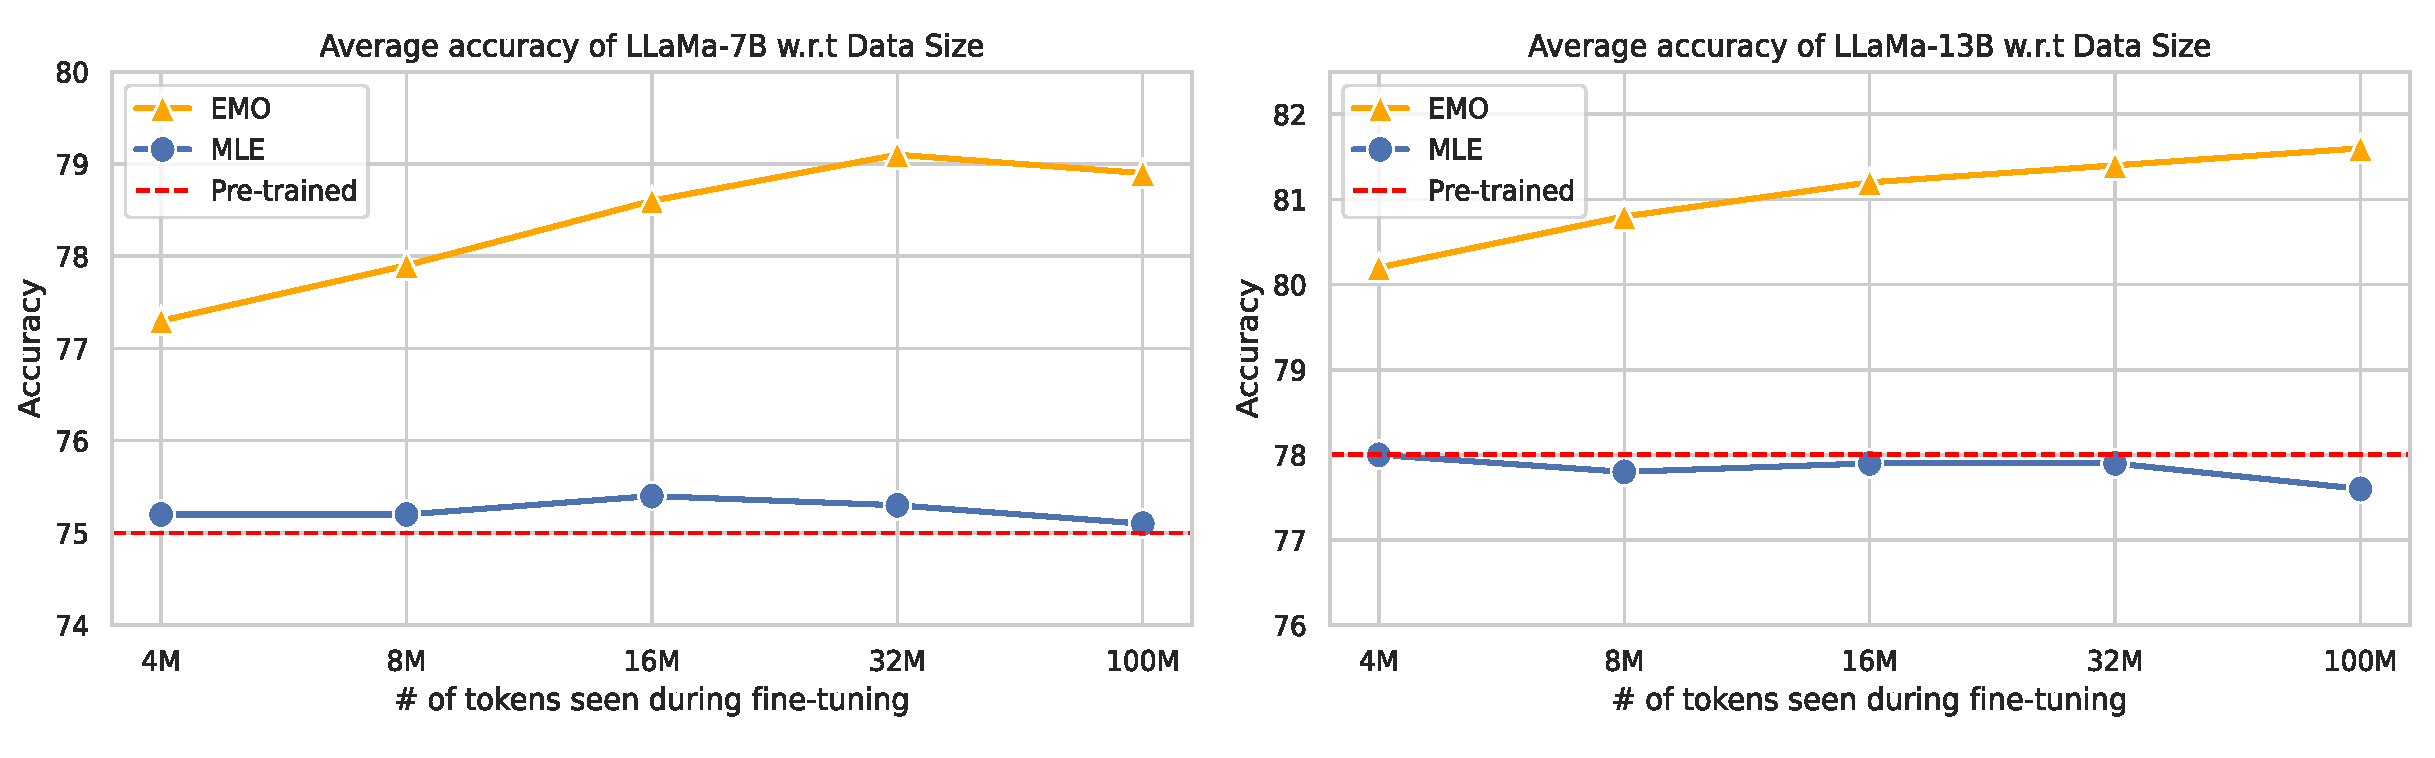
\includegraphics[width=0.99\textwidth]{./figures/scaling.pdf}}
    \scalebox{0.945}{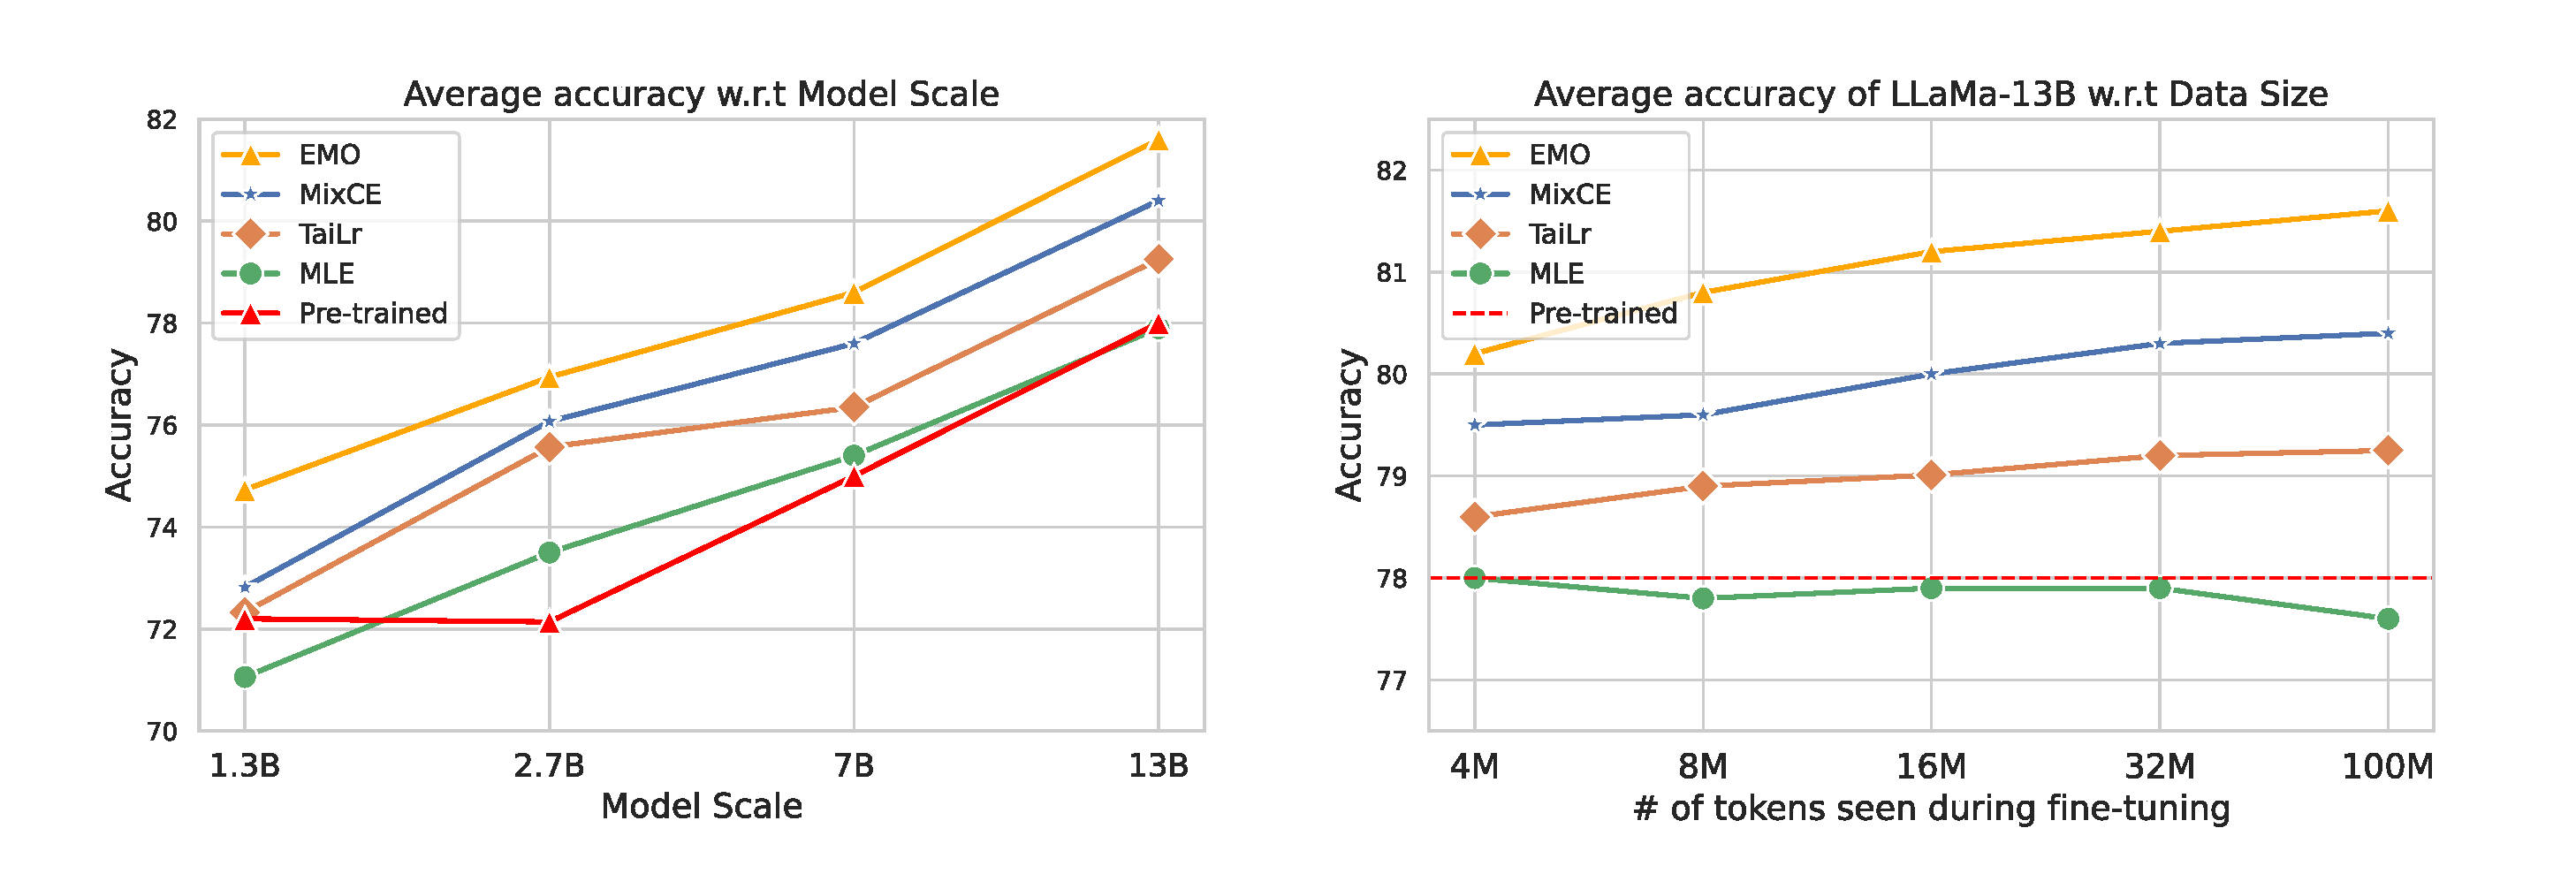
\includegraphics[width=0.99\textwidth]{./figures/main.pdf}}
    % 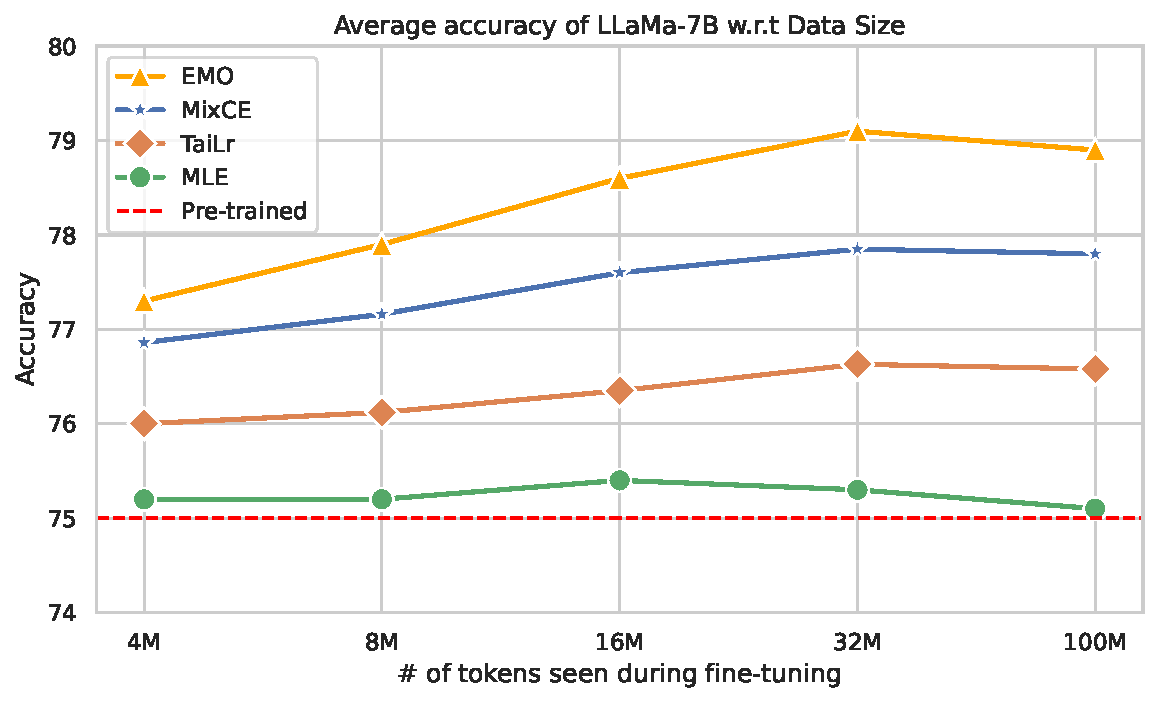
\includegraphics[width=0.49\textwidth]{./figures/scaling_data_7b.pdf}
    % 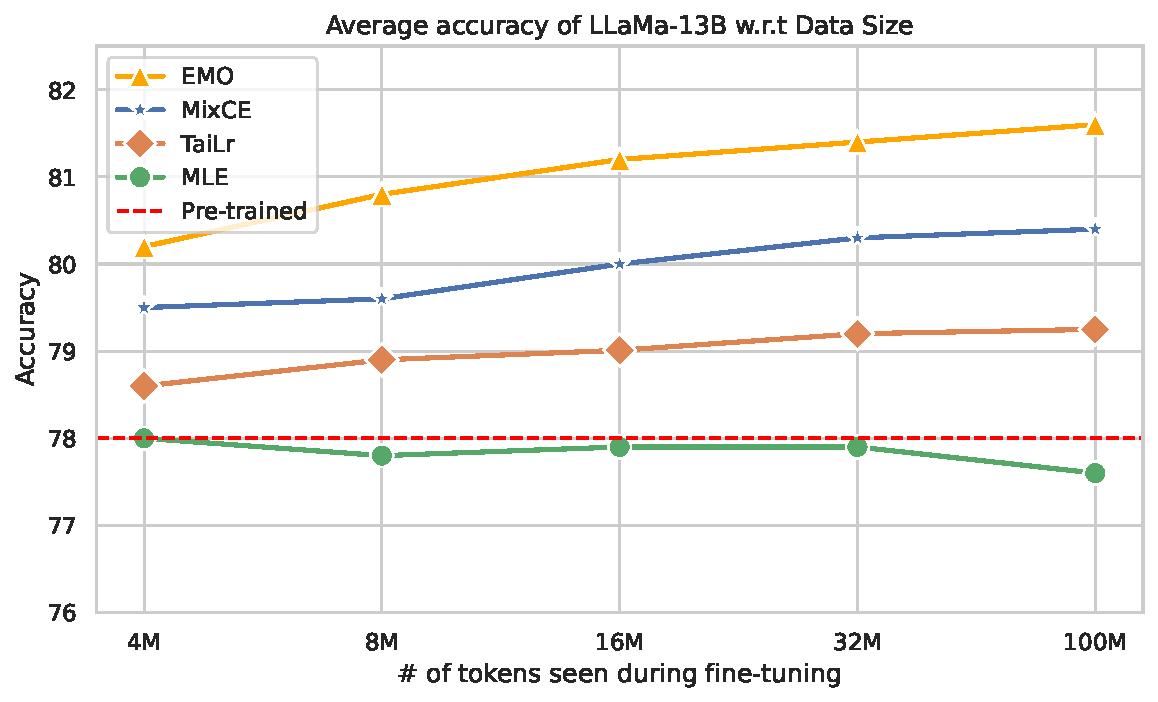
\includegraphics[width=0.49\textwidth]{./figures/scaling_data.pdf}
    \caption{Scaling law of EMO with respect to model scale and data size.}
    \label{fig:scaling}
\end{figure}

\paragraph{Model Scaling} To comprehensively quantify the effectiveness of EMO, we perform the previously described experiment upon OPT-1.3B/2.7B~\citep{opt} in addition to LLaMa-7B/13B and visualize the scaling curve of the task accuracy averaged over the collection of 8 datasets with respect to model scale in Fig.\ref{fig:scaling}~(left). While MLE fails to consistently improve over pre-trained models, TaiLr and MixCE both bring positive impacts when their weighting coefficients are carefully tuned. Notably, EMO shows steady improvements over other methods across all model scales.
\paragraph{Data Scaling} We further examine how performance changes by varying data volumes during fine-tuning. We monitor the change of average accuracy using LLaMa-13B and display the results in Fig.~\ref{fig:scaling}~(right).  
MLE-tuned models exhibit certain declines in accuracy as fine-tuning progresses, which can be attributed to its theoretical deficiencies described in Sec.~\ref{sec:deficiency}. TailLr and MixCE moderately improve over MLE. EMO shows the most significant performance boost and even matches the performance of 100M-tokens-trained MixCE with merely 4M tokens. This highlights the potential of employing EMO in a post-training phase to refine the distribution of pre-trained LLMs for improved downstream performance in an effective and sample-efficient manner.
\label{sec:nlu}